\documentclass[12pt]{article}
\usepackage{amsmath}
\usepackage{amssymb}
\usepackage[spanish]{babel}
\usepackage{mathabx}
\usepackage{geometry}
\usepackage{pdflscape}
\usepackage[demo]{graphicx}
\usepackage{subcaption}

\setcounter{MaxMatrixCols}{20}

\geometry{margin=2cm}

\def\doubleunderline#1{\underline{\underline{#1}}}
\def\diff[#1]#2{\frac{\mathrm{d}#1}{\mathrm{d}#2}}
\def\diffp[#1]#2{\frac{\partial#1}{\partial#2}}
\def\mt#1{\underline{\underline{\mathbf{#1}}}}
\def\d#1{\; \mathrm{d}#1}
\newcommand{\vv}{\vec{v}}
\newcommand{\vf}{\vec{f}}
\newcommand{\vP}{\vec{P}}
\newcommand{\Pb}{\vec{\mathbf{P}}}
\newcommand{\vb}{\vec{\mathbf{v}}}
\newcommand{\nb}{\doubleunderline{\mathbf{N}}}

\title{T\'ecnicas de simulaci\'on por computadora}
\author{Grupo O}
\begin{document}
\maketitle
\vspace{3cm}
\section{Ecuaciones de Navier-Stokes}
\begin{align*}
	\diffp[\vv]{t} + \vv \cdot \nabla (\vv) + \frac{1}{\rho} \nabla P - \nu \nabla \nabla \vv &= \vf \\
	\diffp[\rho]{t} + \rho \nabla \vv &= 0
\end{align*}

\section{Discretizaci\'on espacial en tres dimensiones}

\subsection{Aplicando aproximaci\'on con funciones de forma al vector $\vv$}
Nos basamos en la aproximaci\'on escalar, la cual otorgada una interpolaci\'on lineal
para los valores dentro del elemento que no eran parte de los v\'ertices. En este caso, al ser una
variable vectorial, nos vemos en la necesidad de realizar la aproximaci\'on separando las tres componentes
del vector tridimensional.

\begin{figure}
	\begin{subfigure}{.5\textwidth}
	  \centering
	  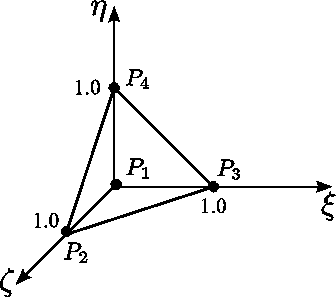
\includegraphics[width=.8\linewidth]{f1.png}
	  \caption{coordenadas isoparam\'etricas}
	\end{subfigure}%
	\begin{subfigure}{.5\textwidth}
	  \centering
	  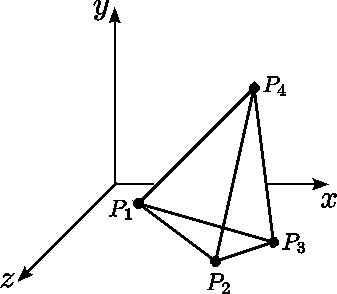
\includegraphics[width=.8\linewidth]{f2.png}
	  \caption{coordenadas cartesianas}
	\end{subfigure}
\end{figure}
\begin{align*}
\vv &\approx \begin{bmatrix} N_1 & N_2 & N_3 & N_4 \end{bmatrix} \begin{bmatrix} \vv_1 \\ \vv_2 \\ \vv_3 \\ \vv_4 \end{bmatrix} = N_1 \vv_1 + N_2 \vv_2 + N_3 \vv_3 + N_4 \vv_4 \\ \\
v^{x} &\approx N_1v^{x}_{1} +  N_2v^{x}_{2} +  N_3v^{x}_{3} +  N_4v^{x}_{4} \\
v^{y} &\approx N_1v^{y}_{1} +  N_2v^{y}_{2} +  N_3v^{y}_{3} +  N_4v^{y}_{4} \\
v^{z} &\approx N_1v^{z}_{1} +  N_2v^{z}_{2} +  N_3v^{z}_{3} +  N_4v^{z}_{4}
\end{align*}

En la matriz de funciones de forma $\nb$ tienen que considerarse t\'erminos nulos para que la multiplicaci\'on tenga el sentido deseado.

\begin{align*}
\vv &\approx \nb \vb \\
\vv_{3 \times 1} & \approx \nb_{3 \times 12} \vb_{12 \times 1}
\\ \\
\vv &\approx	\begin{bmatrix} 
	N_1v^{x}_{1} +  N_2v^{x}_{2} +  N_3v^{x}_{3} +  N_4v^{x}_{4} \\
	N_1v^{y}_{1} +  N_2v^{y}_{2} +  N_3v^{y}_{3} +  N_4v^{y}_{4} \\
	N_1v^{z}_{1} +  N_2v^{z}_{2} +  N_3v^{z}_{3} +  N_4v^{z}_{4}
 \end{bmatrix}
\\
\vb & =
\begin{bmatrix}
	v_{1}^{x} & v_{1}^{y} & v_{1}^{z} &  v_{2}^{x} & v_{2}^{y} & v_{2}^{z} &  v_{3}^{x} & v_{3}^{y} & v_{3}^{z} &  v_{4}^{x} & v_{4}^{y} & v_{4}^{z}
\end{bmatrix}^{T}_{12 \times 1}
\\ \\
\nb &=
\begin{bmatrix}
	N_1 & 0 & 0 &  N_2 & 0 & 0 &  N_3 & 0 & 0 &  N_4 & 0 & 0 \\
	0 & N_1 & 0 & 0 &  N_2 & 0 & 0 &  N_3 & 0 & 0 &  N_4 & 0 \\
	0 & 0 & N_1 & 0 & 0 &  N_2 & 0 & 0 &  N_3 & 0 & 0 &  N_4
\end{bmatrix}_{3 \times 12} \\
\\
N_1 &= 1 - \epsilon - \eta - \zeta \\
N_2 &= \epsilon \\
N_3 &= \eta \\
N_4 &= \zeta \\
\\
\nb &=
\begin{bmatrix}
	1 - \epsilon - \eta - \zeta & 0 & 0 &  \epsilon & 0 & 0 &  \eta & 0 & 0 &  \zeta & 0 & 0 \\
	0 & 1 - \epsilon - \eta - \zeta & 0 & 0 &  \epsilon & 0 & 0 &  \eta & 0 & 0 &  \zeta & 0 \\
	0 & 0 & 1 - \epsilon - \eta - \zeta & 0 & 0 &  \epsilon & 0 & 0 &  \eta & 0 & 0 &  \zeta
\end{bmatrix}
\end{align*}

En el caso de la presi\'on $P$, para lograr consistencia con la dimensi\'on del resto de matrices
ser\'a tratado como un `vector'. Se asignar\'a un promedio de las 3 coordenadas al finalizar los c\'alculos.
\begin{align*}
	\vP &\approx  N_1 \vP_1 + N_2 \vP_2 + N_3 \vP_3 + N_4 \vP_4 \\
	\vP &\approx \nb \Pb \\
	\Pb &= \begin{bmatrix} \frac{P_1}{3} & \frac{P_1}{3} & \frac{P_1}{3} & \frac{P_2}{3} & \frac{P_2}{3} & \frac{P_2}{3} & \frac{P_3}{3} & \frac{P_3}{3} & \frac{P_3}{3} & \frac{P_4}{3} & \frac{P_4}{3} & \frac{P_4}{3} \end{bmatrix}^{T}
\end{align*}

\subsection{Aproximaci\'on de coordenadas espaciales en base a las funciones de forma}
\begin{align*}
	x &= (x_3 - x_1) \epsilon + (x_4 - x_1) \eta  + (x_2 - x_1) \zeta + x_1	 \\
	y &= (y_3 - y_1) \epsilon + (y_4 - y_1) \eta  + (y_2 - y_1) \zeta + y_1	 \\
	z &= (z_3 - z_1) \epsilon + (z_4 - z_1) \eta  + (z_2 - z_1) \zeta + z_1
\end{align*}

\subsection{Derivadas espaciales}
\begin{align*}
	\nabla_{\mt{x}} \; \nb &= \left(\nabla_{\mt{\epsilon}} \; \mt{x} \right)^{-1} \nabla_{\mt{\epsilon}} \; \nb \\ \\
	\mt{x} &= \begin{bmatrix} x & y & z \end{bmatrix} \quad \mt{\epsilon} = \begin{bmatrix} \epsilon & \eta & \zeta \end{bmatrix}
\end{align*}

\begin{align*}
\nabla_{\mt{\epsilon}} \; \mt{x}  &= \begin{bmatrix} \diffp[]{\epsilon} \\ \diffp[]{\eta} \\ \diffp[]{\zeta} \end{bmatrix} \begin{bmatrix} x & y & z \end{bmatrix}
=
\begin{bmatrix}
\diffp[x]{\epsilon} & \diffp[x]{\eta} & \diffp[x]{\zeta} \\
\diffp[y]{\epsilon} & \diffp[y]{\eta} & \diffp[y]{\zeta} \\
\diffp[z]{\epsilon} & \diffp[z]{\eta} & \diffp[z]{\zeta}
\end{bmatrix}
\\
&=
\begin{bmatrix}
	x_3 - x_1 & x_4 - x_1 & x_2 - x_1 \\
	y_3 - y_1 & y_4 - y_1 & y_2 - y_1 \\
	z_3 - z_1 & z_4 - z_1 & z_2 - z_1
\end{bmatrix}
\\ \\
\nabla_{\mt{\epsilon}} \; \nb &= \begin{bmatrix} \diffp[]{\epsilon} \\ \diffp[]{\eta} \\ \diffp[]{\zeta} \end{bmatrix}
\begin{bmatrix}
	N_1 & 0 & 0 &  N_2 & 0 & 0 &  N_3 & 0 & 0 &  N_4 & 0 & 0 \\
	0 & N_1 & 0 & 0 &  N_2 & 0 & 0 &  N_3 & 0 & 0 &  N_4 & 0 \\
	0 & 0 & N_1 & 0 & 0 &  N_2 & 0 & 0 &  N_3 & 0 & 0 &  N_4
\end{bmatrix}
\\
\end{align*}

\begin{align*}
\nabla_{\mt{\epsilon}} \; \nb &=
\begin{bmatrix}
	\diffp[N_1]{\epsilon} & \diffp[N_1]{\epsilon} & \diffp[N_1]{\epsilon} & \diffp[N_2]{\epsilon} & \diffp[N_2]{\epsilon} & \diffp[N_2]{\epsilon} & \diffp[N_3]{\epsilon} & \diffp[N_3]{\epsilon} & \diffp[N_3]{\epsilon} & \diffp[N_4]{\epsilon} & \diffp[N_4]{\epsilon} & \diffp[N_4]{\epsilon} \\ 
	\diffp[N_1]{\eta} & \diffp[N_1]{\eta} & \diffp[N_1]{\eta} & \diffp[N_2]{\eta} & \diffp[N_2]{\eta} & \diffp[N_2]{\eta} & \diffp[N_3]{\eta} & \diffp[N_3]{\eta} & \diffp[N_3]{\eta} & \diffp[N_4]{\eta} & \diffp[N_4]{\eta} & \diffp[N_4]{\eta} \\ 
	\diffp[N_1]{\zeta} & \diffp[N_1]{\zeta} & \diffp[N_1]{\zeta} & \diffp[N_2]{\zeta} & \diffp[N_2]{\zeta} & \diffp[N_2]{\zeta} & \diffp[N_3]{\zeta} & \diffp[N_3]{\zeta} & \diffp[N_3]{\zeta} & \diffp[N_4]{\zeta} & \diffp[N_4]{\zeta} & \diffp[N_4]{\zeta}
\end{bmatrix}
\\
&=
\begin{bmatrix}
	-1 & -1 & -1 & 1 & 1 & 1 & 0 & 0 & 0 & 0 & 0 & 0 \\ 
	-1 & -1 & -1 & 0 & 0 & 0 & 1 & 1 & 1 & 0 & 0 & 0 \\ 
	-1 & -1 & -1 & 0 & 0 & 0 & 0 & 0 & 0 & 1 & 1 & 1
\end{bmatrix}
\\ \\
\nabla_{\mt{x}} \; \nb &=
\begin{bmatrix}
	x_3 - x_1 & x_4 - x_1 & x_2 - x_1 \\
	y_3 - y_1 & y_4 - y_1 & y_2 - y_1 \\
	z_3 - z_1 & z_4 - z_1 & z_2 - z_1
\end{bmatrix}^{-1}
\begin{bmatrix}
	-1 & -1 & -1 & 1 & 1 & 1 & 0 & 0 & 0 & 0 & 0 & 0 \\ 
	-1 & -1 & -1 & 0 & 0 & 0 & 1 & 1 & 1 & 0 & 0 & 0 \\ 
	-1 & -1 & -1 & 0 & 0 & 0 & 0 & 0 & 0 & 1 & 1 & 1
\end{bmatrix}
\end{align*}

\subsection{Aplicaci\'on del m\'etodo de los elementos finitos}
Antes de aplicar el m\'etodo de elementos finitos a las ecuaciones de Navier-Stokes, tendremos en cuenta las siguientes
simplificaciones:
\begin{enumerate}
	\item El t\'ermino de viscosidad $\nu$ y la densidad $\rho$ se mantienen constantes en nuestro modelo.
	\item Por simplicidad, se ignorar\'a el t\'ermino temporal para luego volver a introducirlo en los sistemas de ecuaciones finales.
\end{enumerate}
\begin{align*}
	\diffp[\vv]{t} + \vv \cdot \nabla (\vv) + \frac{1}{\rho} \nabla P - \nu \nabla \nabla \vv - \vf &= 0 \\
	\diffp[\rho]{t} + \rho \nabla \vv &= 0
\end{align*}

Al aplicar el m\'etodo de los residuos ponderados, tendremos dos funciones de peso, $\mt{W_1}$ para la primera ecuaci\'on,
$\mt{W_2}$ para la segunda y sus residuales respectivos $\mathcal{R}_1$ y $\mathcal{R}_2$.
Para simplificar c\'alculos, aplicaremos el m\'etodo de Galerkin, el cual permite el uso
de la matriz transpuesta de funciones de forma como funciones de peso, en nuestro caso $\nb^{T}$. La \textit{forma fuerte}
de nuestra aproximaci\'on de elementos finitos se presenta acontinuaci\'on
\begin{align*}
	\vv \cdot \nabla (\nb \vb) + \frac{1}{\rho} \nabla \nb \Pb - \nu \nabla \nabla (\nb \vb)  -\vf &= \mathcal{R}_1 \\
	\rho \nabla (\nb \vb) &= \mathcal{R}_2 \\
	\\
	\int_{V} \mt{W_1} \left[ \vv \cdot \nabla (\nb \vb) + \frac{1}{\rho} \nabla \nb \Pb - \nu \nabla \nabla (\nb \vb) - \vf \right] \d{V} &= \int_{V} \mt{W_1} \mathcal{R}_1 \d{V} \\
	\int_{V} \mt{W_2} \rho \nabla (\nb \vb) \d{V} &= \int_{V} \mt{W_2} \mathcal{R}_2 \d{V} \\
	\\
	\int_{V} \mt{W_1} \left[ \vv \cdot \nabla (\nb \vb) + \frac{1}{\rho} \nabla \nb \Pb - \nu \nabla \nabla (\nb \vb) - \vf \right] \d{V} &= 0 \\
	\int_{V} \mt{W_2} \rho \nabla (\nb \vb) \d{V} &= 0 \\
	\\
	\int_{V} \nb^{T} \left[ \vv \cdot \nabla (\nb \vb) + \frac{1}{\rho} \nabla \nb \Pb - \nu \nabla \nabla (\nb \vb) - \vf \right] \d{V} &= 0 \\
	\int_{V} \nb^{T} \rho \nabla (\nb \vb) \d{V} &= 0 \\
	\int_{V} \nb^{T} \nabla (\nb \vb) \d{V} &= 0 \\
	\\
	\int_{V} \nb^{T} \left[ \vv \cdot \nabla (\nb \vb) + \frac{1}{\rho} \nabla \nb \Pb - \nu \nabla \nabla (\nb \vb) - \vf + \nabla (\nb \vb) \right] \d{V} &= 0
\end{align*}

Extraemos las constantes mencionadas en las simplificaciones a tomar en cuenta y definimos la convenci\'on de signo de nuestro
sistema de ecuaciones.

\begin{align*}
	\int_{V} \nb \left[ \vv \cdot \nabla (\nb \vb) + \frac{1}{\rho} \nabla \nb \Pb - \nu \nabla \nabla (\nb \vb) - \vf + \nabla (\nb \vb) \right] \d{V} &= 0 \\
	\int_{V} \nb^{T} \vv \cdot \nabla (\nb \vb) \d{V} +  \int_{V} \nb^{T} \frac{1}{\rho} \nabla \nb \Pb \d{V} - \int_{V} \nb^{T} \nu \nabla \nabla (\nb \vb) \d{V} - \int_{V} \nb^{T} \vf \d{V} + \int_{V} \nb^{T} \nabla (\nb \vb) \d{V} &= 0 \\
	\int_{V} \nb^{T} \vv \cdot \nabla \nb \d{V} \vb +  \frac{1}{\rho} \int_{V} \nb^{T} \nabla \nb \d{V} \Pb - \nu \int_{V} \nb^{T}\nabla \nabla \nb \d{V} \vb - \int_{V} \nb^{T} \d{V} \vf + \int_{V} \nb^{T} \nabla \nb \d{V} \vb &= 0 \\
\end{align*}

\newcommand{\A}{\int_{V} \nb^{T} \d{V} \vf}
\newcommand{\B}{\int_{V} \nb^{T} \vv \cdot \nabla \nb  \d{V} \vb}
\newcommand{\C}{\frac{1}{\rho} \int_{V} \nb^{T} \nabla \nb \d{V} \Pb}
\newcommand{\D}{\nu \int_{V} \nb^{T}\nabla \nabla \nb  \d{V} \vb}
\newcommand{\E}{\int_{V} \nb^{T} \nabla \cdot \nb  \d{V} \vb}

Las siguientes ecuaciones representan la \textit{forma fuerte} nuestro sistema, n\'otese la inclusi\'on
de la derivada temporal de la velocidad.
\\
\scalebox{0.95}{\parbox{\linewidth}{%
\begin{align*}
\A - \diffp[\vb]{t} - \B - \C + \D - \E = 0
\end{align*}
}}
\[
	\mt{A} \vf - \diffp[\vb]{t} -\mt{B} \vb - \mt{C} \Pb + \mt{D} \vb - \mt{E} \vb = 0
\]

\newcommand{\NTe}{\left[\begin{matrix}- \epsilon - \eta - \zeta + 1 & 0 & 0\\0 & - \epsilon - \eta - \zeta + 1 & 0\\0 & 0 & - \epsilon - \eta - \zeta + 1\\\epsilon & 0 & 0\\0 & \epsilon & 0\\0 & 0 & \epsilon\\\eta & 0 & 0\\0 & \eta & 0\\0 & 0 & \eta\\\zeta & 0 & 0\\0 & \zeta & 0\\0 & 0 & \zeta\end{matrix}\right]}
\newcommand{\NTesolved}{\left[\begin{matrix}- \frac{1}{2} & 0 & 0\\0 & - \frac{1}{2} & 0\\0 & 0 & - \frac{1}{2}\\\frac{1}{2} & 0 & 0\\0 & \frac{1}{2} & 0\\0 & 0 & \frac{1}{2}\\\frac{1}{2} & 0 & 0\\0 & \frac{1}{2} & 0\\0 & 0 & \frac{1}{2}\\\frac{1}{2} & 0 & 0\\0 & \frac{1}{2} & 0\\0 & 0 & \frac{1}{2}\end{matrix}\right]}
\newcommand{\Ne}{\left[\begin{array}{cccccccccccc}- \epsilon - \eta - \zeta + 1 & 0 & 0 & \epsilon & 0 & 0 & \eta & 0 & 0 & \zeta & 0 & 0\\0 & - \epsilon - \eta - \zeta + 1 & 0 & 0 & \epsilon & 0 & 0 & \eta & 0 & 0 & \zeta & 0\\0 & 0 & - \epsilon - \eta - \zeta + 1 & 0 & 0 & \epsilon & 0 & 0 & \eta & 0 & 0 & \zeta\end{array}\right]}
\newcommand{\deps}{\; \d{\epsilon} \d{\eta} \d{\zeta}}
\newcommand{\inteps}{\int_{0}^{1} \int_{0}^{1} \int_{0}^{1}}
\newcommand{\vfe}{\begin{bmatrix} f_x \\ f_y \\ f_z \end{bmatrix}}
\newcommand{\vbe}{\begin{bmatrix} v_{1}^{x} \\ v_{1}^{y} \\ v_{1}^{z} \\  v_{2}^{x} \\ v_{2}^{y} \\ v_{2}^{z} \\  v_{3}^{x} \\ v_{3}^{y} \\ v_{3}^{z} \\  v_{4}^{x} \\ v_{4}^{y} \\ v_{4}^{z} \end{bmatrix}}
\newcommand{\Pbe}{\begin{bmatrix} \frac{P_1}{3} \\ \frac{P_1}{3} \\ \frac{P_1}{3} \\ \frac{P_2}{3} \\ \frac{P_2}{3} \\ \frac{P_2}{3} \\ \frac{P_3}{3} \\ \frac{P_3}{3} \\ \frac{P_3}{3} \\ \frac{P_4}{3} \\ \frac{P_4}{3} \\ \frac{P_4}{3} \end{bmatrix}}
\newcommand{\Det} {
\begin{vmatrix}
	x_3 - x_1 & x_4 - x_1 & x_2 - x_1 \\
	y_3 - y_1 & y_4 - y_1 & y_2 - y_1 \\
	z_3 - z_1 & z_4 - z_1 & z_2 - z_1
\end{vmatrix}
}
\newcommand{\Dn}{
\begin{bmatrix}
	x_3 - x_1 & x_4 - x_1 & x_2 - x_1 \\
	y_3 - y_1 & y_4 - y_1 & y_2 - y_1 \\
	z_3 - z_1 & z_4 - z_1 & z_2 - z_1
\end{bmatrix}^{-1}
\begin{bmatrix}
	-1 & -1 & -1 & 1 & 1 & 1 & 0 & 0 & 0 & 0 & 0 & 0 \\ 
	-1 & -1 & -1 & 0 & 0 & 0 & 1 & 1 & 1 & 0 & 0 & 0 \\ 
	-1 & -1 & -1 & 0 & 0 & 0 & 0 & 0 & 0 & 1 & 1 & 1
\end{bmatrix}
}
\newcommand{\nbe}{
\begin{bmatrix}
	N_1 & 0 & 0 &  N_2 & 0 & 0 &  N_3 & 0 & 0 &  N_4 & 0 & 0 \\
	0 & N_1 & 0 & 0 &  N_2 & 0 & 0 &  N_3 & 0 & 0 &  N_4 & 0 \\
	0 & 0 & N_1 & 0 & 0 &  N_2 & 0 & 0 &  N_3 & 0 & 0 &  N_4
\end{bmatrix}
}
\newcommand{\gradn}[1]{\diffp[#1]{x} + \diffp[#1]{y} + \diffp[#1]{z}}
\newcommand{\gradnbe}{
\begin{bmatrix}
	\gradn{N_1} & 0 & 0 &  \gradn{N_2} & 0 & 0 &  \gradn{N_3} & 0 & 0 &  \gradn{N_4} & 0 & 0 \\
	0 & \gradn{N_1} & 0 & 0 &  \gradn{N_2} & 0 & 0 &  \gradn{N_3} & 0 & 0 &  \gradn{N_4} & 0 \\
	0 & 0 & \gradn{N_1} & 0 & 0 &  \gradn{N_2} & 0 & 0 &  \gradn{N_3} & 0 & 0 &  \gradn{N_4}
\end{bmatrix}
}
\subsection{Soluci\'on de las integrales}

\begin{align*}
	\mt{A}\vf &= \A  \\
	&= \inteps \left\{\NTe\right\} D \deps \vfe \\
	&= D \NTesolved \vfe \\
	&= \Det \NTesolved \vfe
\end{align*}

\newpage

\begin{landscape}
\scalebox{0.8}{\parbox{\linewidth}{%
\begin{align*}
	\mt{B}\vb &= \B \\
	&= \vv \int_{V} \nb^{T} \nabla \nb \d{VV} \vbe \\
	&= \vv D \inteps \left\{ \NTe \right\} \deps \Dn \vbe \\
	&= \vv \Det \NTesolved \Dn \vbe  \\
\end{align*}
}}
\\
\scalebox{0.8}{\parbox{\linewidth}{%
\begin{align*}
	\mt{C}\Pb &= \C \\
	&= \frac{1}{\rho} \inteps \left\{ \NTe \Dn \right\} D \deps \Pbe \\
	&= \frac{1}{\rho} D \inteps \left\{ \NTe\right\} \deps \Dn  \Pbe \\
	&= \frac{1}{\rho} \Det \NTesolved \Dn  \Pbe
\end{align*}
}}
\\
\scalebox{0.8}{\parbox{\linewidth}{%
\begin{align*}
	\mt{D}\vb &= \D \\
	&= \nu \int_{V} \nb^{T} \nabla^2 \nb \d{V} \vb \\
	&= \nu \int_{V} \nb^{T} \Delta \nb \d{V} \vb \\
\end{align*}
}}
\\
\scalebox{0.8}{\parbox{\linewidth}{%
\begin{align*}
	\mt{E}\vb &= \E \\ \\
	\nabla \cdot \nb &=
	\begin{bmatrix}
		\diffp[]{x} \\
		\diffp[]{y} \\
		\diffp[]{z}
	\end{bmatrix}
	\cdot
	\nbe
\end{align*}
}}
\\
\scalebox{0.6}{\parbox{\linewidth}{%
\begin{align*}
	\nabla \cdot \nb &= \gradnbe
\end{align*}
}}
\end{landscape}
\end{document}